\begin{figure}[ht!]
\centering

\scalebox{0.70}{
\begin{tikzpicture}[auto]

% operations =============================

% nodes
\node (original)
    {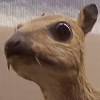
\includegraphics[width=.15\textwidth]{images/Vd-Orig.png}};
\node[above right= 20pt and 150pt of original] (edge) {
\includegraphics[width=.15\textwidth]{images/Vd-Edge3.png}};
\node[below=20pt of edge] (sharpen) {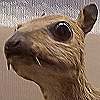
\includegraphics[width=.15\textwidth]{images/Vd-Sharp.png}};
\node[below=20pt of sharpen] (blur) {
\includegraphics[width=.15\textwidth]{images/Vd-Blur1.png}};

% edges
\path[tedge, orange!120, line width=1mm]  (original) to [out=90,in=180, looseness=9, distance=125pt] (edge);
\path[tedge, orange!120, line width=1mm]  (original) to [out=0,in=180] (sharpen);
\path[tedge, orange!120, line width=1mm]  (original) to [out=-90,in=180, looseness=9, distance=125pt] (blur);

% nodes for kernels 
\node[op3, right=20pt of original] (kernel1) {$\begin{bmatrix}0 & -1 & 0\\ -1 & 5 & -1\\0 & -1 & 0\end{bmatrix}$};
\node[op3, above=10pt of kernel1] (kernel2) {$\begin{bmatrix}-1 & -1 & -1\\ -1 & 8 & -1\\-1 & -1 & -1\end{bmatrix}$};
\node[op3, below=10pt of kernel1] (kernel3) {$\frac{1}{16}\begin{bmatrix}1 & 2 & 1\\ 2 & 4 & 2\\1 & 2 & 1\end{bmatrix}$};

\end{tikzpicture}
} % scalebox
\vspace*{-10mm}
\caption{Exemplo de aplicação de filtros em uma imagem (extraído de \url{https://en.wikipedia.org/wiki/Kernel_(image_processing)})}
\end{figure}
